\documentclass[tikz, border=10pt]{standalone}

\usepackage{tikz}
\usepackage{xcolor}

\definecolor{golden}{HTML}{ffd700}

\begin{document}
    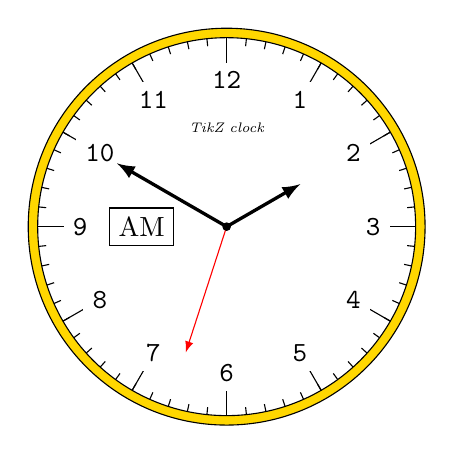
\begin{tikzpicture}[scale=1.2]
        % draw ring of the clock
        \path[draw=black, fill=golden] (0, 0) circle (2.1);
        \path[draw=black, fill=white] (0, 0) circle (2);
        % mark minutes
        \foreach \i in {6, 12, 18, ..., 360}{
            \draw (\i:1.92) -- (\i:2);
        }
        % mark hours
        \foreach \i in {0, 30, 60, ..., 360}{
            \draw (\i:1.4) -- (\i:2);
        }
        % add hour number
        \foreach \i [count=\inc from 1] in {
            60, 30, 0, -30, -60, -90, -120, -150, -180, -210, -240, 90
        }{
            \draw (\i:1.55) node[fill=white] {\texttt{\inc}};
        }
        % add text labels
        \draw (90:1.05) node {\it\tiny{TikZ clock}};
        \draw (180:0.9) node[fill=white, draw=black] {AM};
        % draw hands
        \draw[very thick, -latex] (0, 0) -- (150:1.34);
        \draw[very thick, -latex] (0, 0) -- (30:0.9);
        \draw[thin, red, -latex] (0, 0) -- (-108:1.4);
        \fill[black] (0, 0) circle (1.3pt);
    \end{tikzpicture}
\end{document}